\PassOptionsToPackage{unicode=true}{hyperref} % options for packages loaded elsewhere
\PassOptionsToPackage{hyphens}{url}
%
\documentclass[10pt,xcolor=table,color={dvipsnames,usenames},ignorenonframetext,usepdftitle=false,french]{beamer}
\setbeamertemplate{caption}[numbered]
\setbeamertemplate{caption label separator}{: }
\setbeamercolor{caption name}{fg=normal text.fg}
\beamertemplatenavigationsymbolsempty
\usepackage{caption}
\captionsetup{skip=0pt,belowskip=0pt}
%\setlength\abovecaptionskip{-15pt}
\usepackage{lmodern}
\usepackage{amssymb,amsmath,mathtools,multirow}
\usepackage{float,hhline}
\usepackage{tikz}
\usepackage{mathtools}
\usepackage{ifxetex,ifluatex}
\usepackage{fixltx2e} % provides \textsubscript
\ifnum 0\ifxetex 1\fi\ifluatex 1\fi=0 % if pdftex
  \usepackage[T1]{fontenc}
  \usepackage[utf8]{inputenc}
  \usepackage{textcomp} % provides euro and other symbols
\else % if luatex or xelatex
  \usepackage{unicode-math}
  \defaultfontfeatures{Ligatures=TeX,Scale=MatchLowercase}
\fi
\usetheme[coding=utf8,language=french,
,titlepagelogo=img/logobeamer.png
]{TorinoTh}
% use upquote if available, for straight quotes in verbatim environments
\IfFileExists{upquote.sty}{\usepackage{upquote}}{}
% use microtype if available
\IfFileExists{microtype.sty}{%
\usepackage[]{microtype}
\UseMicrotypeSet[protrusion]{basicmath} % disable protrusion for tt fonts
}{}
\IfFileExists{parskip.sty}{%
\usepackage{parskip}
}{% else
\setlength{\parindent}{0pt}
\setlength{\parskip}{6pt plus 2pt minus 1pt}
}
\usepackage{hyperref}
\hypersetup{
            pdftitle={Real-time detection of turning points with linear filters},
            pdfauthor={Alain Quartier-la-Tente},
            pdfborder={0 0 0},
            breaklinks=true}
\urlstyle{same}  % don't use monospace font for urls
\newif\ifbibliography
% Prevent slide breaks in the middle of a paragraph:
\widowpenalties 1 10000
\raggedbottom
\AtBeginPart{
  \let\insertpartnumber\relax
  \let\partname\relax
  \frame{\partpage}
}
\setlength{\emergencystretch}{3em}  % prevent overfull lines
\providecommand{\tightlist}{%
  %\setlength{\itemsep}{0pt}
  \setlength{\parskip}{0pt}
  }
\setcounter{secnumdepth}{0}

% set default figure placement to htbp
\makeatletter
\def\fps@figure{htbp}
\makeatother

\usepackage{dsfont}
\usepackage{stmaryrd}
\usepackage[normalem]{ulem}
\usepackage{fontawesome5}
\usepackage{tikz,pgfplots}
\pgfplotsset{compat=1.17}
\pgfplotsset{samples=100}
\usepackage{animate}


\DeclareMathOperator{\Cov}{Cov}
\newcommand{\cov}[2]{\Cov\left( #1\,,\,#2 \right)}

\DeclareMathOperator{\e}{e}
\renewcommand{\P}{\mathds{P}} %Apparement \P existe déjà ?
\newcommand\N{\mathds{N}}
\newcommand\R{\mathds{R}}


\newcommand\1{\mathds{1}}
\newcommand{\E}[2][]{{\mathds{E}}_{#1}
  \def\temp{#2}\ifx\temp\empty
  \else
    \left[#2\right]
  \fi
}
\newcommand{\V}[2][]{{\mathds{V}}_{#1}
  \def\temp{#2}\ifx\temp\empty
  \else
    \left[#2\right]
  \fi
}
\newcommand\ud{\,\mathrm{d}}


% blocks
\usepackage{environ}
\usepackage[tikz]{bclogo}

\tikzstyle{titlestyle} =[draw=black!80,fill=black!20, text=black,
 right=10pt, rounded corners]
\mdfdefinestyle{symmaryboxstyle}{
	linecolor=black!80, backgroundcolor = black!5,
	skipabove=\baselineskip, innertopmargin=\baselineskip,
	innerbottommargin=\baselineskip,
	userdefinedwidth=\textwidth,
	middlelinewidth=1.2pt, roundcorner=5pt,
	skipabove={\dimexpr0.5\baselineskip+\topskip\relax},
	frametitleaboveskip=\dimexpr-\ht\strutbox\relax,
	innerlinewidth=0pt,
}
\NewEnviron{summary}{%
\begin{mdframed}[style=symmaryboxstyle]
\vspace{-0.5em}
\BODY
\end{mdframed}
}

\title{Real-time detection of turning points with linear filters}
\ateneo{Stage d'application (2A)}
\author{Alain Quartier-la-Tente}
\date{}


\setrellabel{}

\setcandidatelabel{}

\rel{}
\division{Maître de stage : \textsc{Jean PALATE} (NBB)\\
07/01/2021}

\departement{Ensae --- 2019-2020}
\makeatletter
\let\@@magyar@captionfix\relax
\makeatother


\begin{document}
\begin{frame}[plain,noframenumbering]
\titlepage
\end{frame}

\hypertarget{introduction}{%
\section{Introduction}\label{introduction}}

\begin{frame}[fragile]{Contexte}
\protect\hypertarget{contexte}{}
\begin{itemize}
\tightlist
\item
  Stage de 10 semaines effectué dans la cellule Recherche et
  Développement de la Banque Nationale de Belgique auprès de Jean PALATE
  (NBB)
\end{itemize}

\bigskip

\begin{itemize}
\tightlist
\item
  Stage co-dirigé par Dominique LADIRAY (Insee)
\end{itemize}

\bigskip

\begin{itemize}
\item
  \textbf{Objectif} : préparer une thèse sur l'utilisation des filtres
  asymétriques pour la détection des points de retournement

  \begin{itemize}
  \item
    Première revue de la bibliographie
  \item
    Prise en main de quelques programmes \faIcon{r-project}
    (\texttt{rjdfilters}, \url{https://github.com/palatej/rjdfilters})
  \end{itemize}
\end{itemize}
\end{frame}

\begin{frame}{Introduction (1/2)}
\protect\hypertarget{introduction-12}{}
\begin{itemize}
\tightlist
\item
  Dans l'analyse de la conjoncture, la détection rapide des points de
  retournement est très importante
\end{itemize}

\bigskip
\pause

\begin{itemize}
\tightlist
\item
  Une série \(X_t\) se décompose en plusieurs composantes inobservées :
  \[
  X_t=T_t+C_t+S_t+I_t
  \]
\end{itemize}

\pause

\faArrowCircleRight{} Méthodes d'extraction de
\textbf{tendance}/\textbf{cycle} (\(C_t\) ou \(T_t+C_t\)) liées aux
méthodes de désaisonnalisation

\begin{figure}[!ht]
\pgfplotsset{width=\textwidth,height=3cm,every axis legend/.append style={font=\footnotesize,
  at={(0.5,-0.1)},
  anchor=north}
    }
    \begin{animateinline}[loop,controls]{2}
        \multiframe{19}{rangle=0.1+0.1}{
\begin{tikzpicture}
\begin{axis}[
xtick={0,3.14159,...,15.70795},
xticklabels={0,$10$,$20$,$30$,$40$,$50$}
]
\addplot[domain=0:3*pi,smooth]    plot (\x,{sin(\x r)});
\addplot[domain=(0.314):(\rangle*pi),smooth, color = red, samples = 100]    plot (\x,{sin(\x r)});
\draw[<->, color = red] (axis cs: \rangle*pi-pi/10, {sin((\rangle*pi-pi/10) r)})--(axis cs: \rangle*pi, {sin(\rangle*pi r)});
\draw[<->, color = red] (axis cs: \rangle*pi, {sin(\rangle*pi r)})--(axis cs: \rangle*pi+pi/10, {sin((\rangle*pi+pi/10) r)});
\end{axis}
\end{tikzpicture}
        }
    \end{animateinline}
\end{figure}
\end{frame}

\begin{frame}{Introduction (2/2)}
\protect\hypertarget{introduction-22}{}
\emph{Moyennes mobiles} (ou \emph{filtres linéaires}) omniprésentes dans
ces méthodes (ex : X-12ARIMA)\\
Mathématiquement, à la date \(t\) on calcule : \[
M_\theta(X_t)=\sum_{k=-p}^{+f}\theta_kX_{t+k}
\]

\pause \bigskip

\faArrowCircleRight{} Généralement utilisation de moyennes
\emph{symétriques} (\(p=f\) et \(\theta_{-i}=\theta_i\))

\bigskip

\faArrowCircleRight{} En fin de période, utilisation de méthodes
\emph{asymétriques} : révisions

\pause

\bigskip

\faArrowCircleRight{} Étude des méthodes non-paramétriques qui peuvent
s'intégrer dans X-12-ARIMA et dans le logiciel de désaisonnalisation
JDemetra+ (maintenu par la NBB).
\end{frame}

\hypertarget{propriuxe9tuxe9s-guxe9nuxe9rales-des-moyennes-mobiles}{%
\section{Propriétés générales des moyennes
mobiles}\label{propriuxe9tuxe9s-guxe9nuxe9rales-des-moyennes-mobiles}}

\begin{frame}[noframenumbering]{Sommaire}
\protect\hypertarget{sommaire}{}
\tableofcontents[currentsection, hideothersubsections]
\end{frame}

\hypertarget{gain-et-duxe9phasage}{%
\subsection{Gain et déphasage}\label{gain-et-duxe9phasage}}

\begin{frame}{Gain et déphasage}
\protect\hypertarget{gain-et-duxe9phasage-1}{}
Appliquer \(M_\theta\) sur \(X_t=\sin(\omega t)\) va avoir deux effets :

\begin{enumerate}
\tightlist
\item
  Multiplier le niveau par \(G_{\theta}\left(\omega\right)\)
  (\emph{gain})\\
\item
  Créer un \emph{déphasage} \(\Phi_\theta(\omega)/\omega\) : affecte
  détection des points de retournement
\end{enumerate}

Exemple :

\(\,M_{\theta_0}X_t=\frac{1}{2}X_{t-1}+\frac{1}{2}X_{t},\,\omega=\pi/2\)

\begin{figure}[!ht]
\pgfplotsset{width=\textwidth,height=4cm,every axis legend/.append style={font=\footnotesize,
  at={(0.5,-0.1)},
  anchor=north}
    }
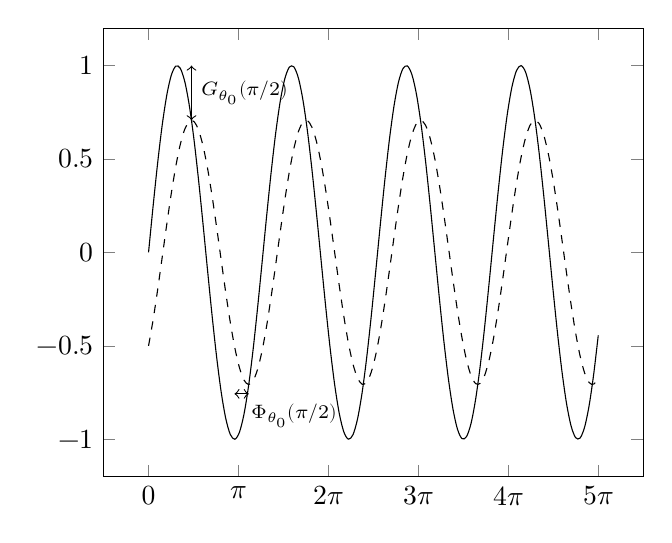
\begin{tikzpicture}
\begin{axis}[
xtick={0,3.14159,...,15.70795},
xticklabels={0,$\pi$,$2\pi$,$3\pi$,$4\pi$,$5\pi$} 
]
\addplot[domain=0:5*pi,smooth]    plot (\x,{sin(\x * (pi/2) r)});
\addplot[domain=0:5*pi,smooth, dashed]    
  plot (\x,{1/2*sin(\x* pi/2 r )+1/2*sin((\x -1) * pi/2 r)});
\draw[<->](axis cs: 1.5,1)--(axis cs: 1.5,0.7071068)
  node[pos=0.5, right]{\scriptsize $G_{\theta_0}(\pi/2)$};
\draw[<->] (axis cs: 3, -0.70710680-0.05)--(axis cs: 3.5,-0.7071068-0.05) 
  node[pos=0.5, below right]{\scriptsize $\Phi_{\theta_0}(\pi/2)$};
\end{axis}
\end{tikzpicture}
\end{figure}

\pause

\faArrowCircleRight{} Déphasage nul pour MM symétriques
\end{frame}

\hypertarget{conservation-des-tendances-polynomiales}{%
\subsection{Conservation des tendances
polynomiales}\label{conservation-des-tendances-polynomiales}}

\begin{frame}{Conservation des tendances polynomiales}
\protect\hypertarget{conservation-des-tendances-polynomiales-1}{}
\[
X_t=TC_t+\varepsilon_t\implies M_\theta X_t =M_\theta TC_t+M_\theta \varepsilon_t
\]

Généralement tendance approchée par une tendance polynomiale

\faArrowCircleRight{} Contraintes supplémentaires pour les conserver.\\
\pause Exemple :

\begin{itemize}
\tightlist
\item
  \(M_\theta\) conserve les constantes si : \[
  M_\theta(a)=a\implies \sum_{k=-p}^{+f}\theta_k = 1
  \]
\end{itemize}
\end{frame}

\hypertarget{autres-indicateurs}{%
\subsection{Autres indicateurs}\label{autres-indicateurs}}

\begin{frame}{Autres indicateurs}
\protect\hypertarget{autres-indicateurs-1}{}
\begin{enumerate}
\tightlist
\item
  Réduction de la variance (\emph{Fidelity}) : \[
  \V{M_\theta\varepsilon_t}=
  \V{\varepsilon_t}\underbrace{\sum_{k=-p}^{+f} \theta_k^2}_{=F_g}
  \]\\
\item
  Lissage (\emph{Smoothness}) défini par Henderson : \[
  S_G=\sum_{j}(\nabla^{3}\theta_{j})^{2}
  \]
\item
  Temporalité (\emph{Timeliness}) qui mesure le déphasage dans les
  fréquences liées au cycle : \[
   T_{g} =\int_{0}^{2\pi/12}\rho_{\theta}(\omega)\sin(\varphi_{\theta}(\omega))^{2}\ud\omega
  \]
\item
  D'autres critères définis par Wildi et McElroy (2019) en décomposant
  l'erreur quadratique moyenne des révisions : \(A_w\), \(T_w\),
  \(S_w\), \(R_w\).
\end{enumerate}
\end{frame}

\hypertarget{muxe9thodes-de-construction-des-filtres-asymuxe9triques}{%
\section{Méthodes de construction des filtres
asymétriques}\label{muxe9thodes-de-construction-des-filtres-asymuxe9triques}}

\begin{frame}[noframenumbering]{Sommaire}
\protect\hypertarget{sommaire-1}{}
\tableofcontents[currentsection, hideothersubsections]
\end{frame}

\hypertarget{polynuxf4mes-locaux}{%
\subsection{Polynômes Locaux}\label{polynuxf4mes-locaux}}

\begin{frame}{Approche générale, Proietti and Luati (2008)}
\protect\hypertarget{approche-guxe9nuxe9rale-proietti-and-luati-2008}{}
On suppose que l'on peut décomposer notre série
\(y_t=\mu_t+\varepsilon_t\) avec
\(\varepsilon_t\overset{i.i.d}{\sim}\mathcal N(0,\sigma^2)\)

\(\mu_t\) est localement approché par un polynôme de degré \(d\) : \[
\forall j\in\left\llbracket -h,h\right\rrbracket \::\: y_{t+j}=m_{t+j}+\varepsilon_{t+j},\quad m_{t+j}=\sum_{i=0}^{d}\beta_{i}j^{i}
\] \pause Estimation par moindres carrés pondérés (WLS) en minimisant:
\[
S(\hat{\beta}_{0},\dots,\hat{\beta}_{d})=\sum_{j=-h}^{h}\kappa_{j}(y_{t+j}-\hat{\beta}_{0}-\hat{\beta}_{1}j-\dots-\hat{\beta}_{d}j^{d})^{2}
\] \(\kappa_j\) sont les \emph{noyaux}.

\pause

L'estimateur est \(\hat{\beta}=(X'KX)^{1}X'Ky\) et : \[
\hat{m}_{t}=\hat\beta_0=w'y=\sum_{j=-h}^{h}w_{j}y_{t-j}
\text{ \faArrowCircleRight{} estimation par filtre symétrique.}
\]
\end{frame}

\begin{frame}{Construction des filtres asymétriques}
\protect\hypertarget{construction-des-filtres-asymuxe9triques}{}
Plusieurs solutions :

\begin{enumerate}
\tightlist
\item
  Même méthode avec moins de points (DAF) : \textbf{sans biais} mais
  beaucoup de variance
\end{enumerate}

\pause

\begin{enumerate}
\setcounter{enumi}{1}
\item
  Compromis biais-variance : minimisation des révisions sous contraintes
  plus faibles\\
  Filtres \(v\) dépend d'un paramètre à définir par l'utilisateur

  \begin{enumerate}
  \item
    \emph{Linear-Constant} (LC) : \(y_t\) linéaire et \(v\) conserve
    constante
  \item
    \emph{Quadratic-Linear} (QL) : \(y_t\) degré \(2\) et \(v\) conserve
    polynôme degré \(1\)
  \item
    \emph{Cubic-Quadratic} (CQ) : \(y_t\) degré \(3\) et \(v\) conserve
    polynôme degré \(2\)
  \end{enumerate}
\end{enumerate}

\pause

\faDesktop{} Pour visualiser les différentes méthodes :

\url{https://aqlt.shinyapps.io/FiltersProperties/}
\end{frame}

\begin{frame}{Premières analyses}
\protect\hypertarget{premiuxe8res-analyses}{}
\begin{summary}

\begin{itemize}
\tightlist
\item
  \bcsmbh{} Méthode \textbf{simple} qui permet de retrouver les
  principales moyennes mobiles (Henderson, Musgrave, Loess, etc.).
\end{itemize}

\pause

\begin{itemize}
\tightlist
\item
  \bcsmmh{} \textbf{Déphasage non contrôlé} avec parfois des résultats
  étonnants\\
  \onslide<3->{$\rightarrow$ possibilité de changer le programme pour le contrôler}
\end{itemize}

\end{summary}

\onslide<4->{
\begin{itemize}
\item Privilégier LC ou QL qui réduisent les révisions avec un ajout limité du déphasage.
\onslide<5->{\faArrowCircleRight{} se concentrer sur les filtres asymétriques qui preservent les polynômes de degré au plus 1}
\end{itemize}
}
\end{frame}

\hypertarget{minimisation-sous-contrainte-approche-fst}{%
\subsection{Minimisation sous contrainte : approche
FST}\label{minimisation-sous-contrainte-approche-fst}}

\begin{frame}{L'approche FST, Grun-Rehomme et al (2018)}
\protect\hypertarget{lapproche-fst-grun-rehomme-et-al-2018}{}
Minimisation sous contrainte d'une somme pondérée de 3 critères :

\[
\begin{cases}
\underset{\theta}{\min} & J(\theta)=
\alpha F_g(\theta)+\beta S_g(\theta)+\gamma T_g(\theta)\\
s.c. & C\theta=a
\end{cases}
\] \pause

\begin{summary}

\begin{itemize}
\item
  \bcsmbh Avantages :

  \begin{itemize}
  \item
    Solution unique connue analytiquement
  \item
    Filtres asymétriques indépendants des données et du filtre
    symétrique
  \item
    Outil utile pour évaluer les autres méthodes
  \end{itemize}
\item
  \bcsmmh Inconvénient :

  \begin{itemize}
  \tightlist
  \item
    Poids non normalisés
  \end{itemize}
\end{itemize}

\end{summary}
\end{frame}

\hypertarget{filtres-et-reproducing-kernel-hilbert-space-rkhs}{%
\subsection{Filtres et Reproducing Kernel Hilbert Space
(RKHS)}\label{filtres-et-reproducing-kernel-hilbert-space-rkhs}}

\begin{frame}{Filtres RKHS : Dagum and Bianconcini (2008)}
\protect\hypertarget{filtres-rkhs-dagum-and-bianconcini-2008}{}
\begin{itemize}
\tightlist
\item
  Utilisation de la théorie des RKHS pour approximer le filtre de
  Henderson
\end{itemize}

\begin{itemize}
\tightlist
\item
  Avec \(K_p\) la \textbf{fonction de noyau}, le filtre symétrique : \[
  \forall j\in\left\llbracket -h,h\right\rrbracket\::\: w_{j}=\frac{K_p(j/b)}{\sum_{i=-h}^{^h}K_p(i/b)}
  \] Avec \(b=h+1\) on retrouve les filtres polynomiaux locaux
\end{itemize}

\pause

\begin{itemize}
\tightlist
\item
  Pour les filtres asymétriques : \[
  \forall j\in\left\llbracket -h,q\right\rrbracket\::\: w_{a,j}=\frac{K_p(j/b)}{\sum_{i=-h}^{^q}K_p(i/b)}
  \]
\end{itemize}
\end{frame}

\begin{frame}{Filtres asymétriques}
\protect\hypertarget{filtres-asymuxe9triques}{}
\(b\) déterminé par optimisation en minimisant :

\begin{itemize}
\item
  les révisions :
  \(b_{q,\gamma}=\underset{b_q\in]h;2 h+1]}{\min} \sqrt{2\int_{0}^{\pi} \lvert \Gamma_s(\omega)-\Gamma_\theta(\omega)\rvert^2\ud \omega }\)
\item
  les révisions liées à la fonction de gain
  \(b_{q,G}=\underset{b_q\in]h;2 h+1]}{\min} \sqrt{2\int_{0}^{\pi} \left(\rho_s(\omega)-\rho_\theta(\omega)\right)^{2}\ud \omega }\)
\item
  les révisions liées au déphasage
  \(b_{q,\varphi}=\underset{b_q\in]h;2 h+1]}{\min} 8\int_{0}^{2\pi/12} \rho_s(\lambda)\rho_\theta(\lambda)\sin^{2}\left(\frac{\varphi_\theta(\omega)}{2}\right)\ud \omega\)
\end{itemize}
\end{frame}

\begin{frame}{Avantages et inconvénients}
\protect\hypertarget{avantages-et-inconvuxe9nients}{}
\begin{summary}

\begin{itemize}
\item
  \bcsmbh Avantages :

  \begin{itemize}
  \tightlist
  \item
    Méthode généralisable à des filtres avec fréquences irrégulières
  \end{itemize}
\item
  \bcsmmh Inconvénients :

  \begin{itemize}
  \item
    MM ne conservent que les constantes
  \item
    Il peut y avoir des problèmes d'optimisation (plusieurs minimums,
    etc.)
  \end{itemize}
\end{itemize}

\end{summary}
\end{frame}

\hypertarget{comparaison-des-muxe9thodes}{%
\section{Comparaison des méthodes}\label{comparaison-des-muxe9thodes}}

\begin{frame}[noframenumbering]{Sommaire}
\protect\hypertarget{sommaire-2}{}
\tableofcontents[currentsection, hideothersubsections]
\end{frame}

\hypertarget{comparaison-thuxe9orique}{%
\subsection{Comparaison théorique}\label{comparaison-thuxe9orique}}

\begin{frame}{Comparaison à partir de la méthode FST}
\protect\hypertarget{comparaison-uxe0-partir-de-la-muxe9thode-fst}{}
On regarde si on peut faire \textbf{mieux sur les trois critères} avec
la méthode FST et \textbf{mêmes contraintes polynomiales} :\\
\faDesktop{} \url{https://aqlt.shinyapps.io/FSTfilters/}

\pause

\begin{itemize}
\item
  Meilleurs résultats avec FST qu'avec RKHS avec \textbf{mêmes
  contraintes polynomiales}
\item
  Meilleurs résultats avec FST qu'avec LC, sauf lorsque l'on contrôle le
  déphasage pour \(q=0,1\)
\item
  Pas de meilleur résultat avec FST qu'avec QL pour \(q=0,1\)
\end{itemize}
\end{frame}

\hypertarget{comparaison-sur-un-exemple}{%
\subsection{Comparaison sur un
exemple}\label{comparaison-sur-un-exemple}}

\begin{frame}{Un exemple d'application : IPI-FR CL1 (1/2)}
\protect\hypertarget{un-exemple-dapplication-ipi-fr-cl1-12}{}
\animategraphics[controls, height = 0.8\paperheight]{2}{img/illustrationBeamer/illustration_}{1}{5}
\end{frame}

\hypertarget{conclusion}{%
\section{Conclusion}\label{conclusion}}

\begin{frame}[noframenumbering]{Sommaire}
\protect\hypertarget{sommaire-3}{}
\tableofcontents[currentsection, hideothersubsections]
\end{frame}

\begin{frame}{Conclusion}
\protect\hypertarget{conclusion-1}{}
\begin{itemize}
\tightlist
\item
  DAF (utilisé dans STL) donne les moins bons résultats sur détection
  des points de retournement et révisions
\end{itemize}

\bigskip

\begin{itemize}
\tightlist
\item
  Minimiser timeliness n'implique pas une détection plus rapide de tous
  les points de retournement
\end{itemize}

\bigskip

\begin{itemize}
\tightlist
\item
  Introduire du biais dans la préservation des tendances polynomiales
  permet d'améliorer la détection rapide des points de retournement
\end{itemize}

\bigskip \pause

\begin{itemize}
\tightlist
\item
  À partir de \(q=2\) les méthodes donnent des résultats similaires
\end{itemize}
\end{frame}

\begin{frame}{Ouverture}
\protect\hypertarget{ouverture}{}
\begin{itemize}
\tightlist
\item
  Filtres FST permettent de construire des filtres ``meilleurs'' que les
  autres
\end{itemize}

\bigskip \pause

\begin{itemize}
\tightlist
\item
  Beaucoup de paramètres : lesquels sont pertinents ?
\end{itemize}

\bigskip \pause

\begin{itemize}
\tightlist
\item
  Quid de la longueur des filtres et des séries avec d'autres fréquences
  ?
\end{itemize}

\bigskip \pause

\begin{itemize}
\tightlist
\item
  Quid de l'impact des points atypiques : étude des méthodes robustes
\end{itemize}
\end{frame}

\begin{frame}[noframenumbering]{Merci pour votre attention}
\protect\hypertarget{merci-pour-votre-attention}{}
\href{https://github.com/AQLT/AsymmetricFilters}{\faGithub{} AQLT/AsymmetricFilters}

\href{https://aqlt.github.io/AsymmetricFilters/Rapport\%20de\%20stage/Rapport.pdf}{\faEdit{} Rapport du projet}

\href{https://aqlt.github.io/AsymmetricFilters/Rapport\%20de\%20stage/Rapport.pdf}{\faFilePowerpoint{} Slides}

\href{https://github.com/palatej/rjdfilters}{\faRProject \faCube{} palatej/rjdfilters}
\end{frame}

\begin{frame}[noframenumbering]{Annexe 1}
\protect\hypertarget{annexe-1}{}
\animategraphics[controls, width = \textwidth]{2}{img/illustration/est_tr_}{1}{7}
\end{frame}

\end{document}
